\documentclass[8pt,a4paper]{beamer}
\usepackage[utf8]{inputenc}
\usepackage[spanish, es-tabla]{babel}
\usepackage{amsmath}
\usepackage{amsfonts}
\usepackage{amssymb}
\usepackage{graphicx}
\usepackage{extarrows} 
\usepackage{multirow}
\usepackage{ragged2e}
\usepackage{mathrsfs}
\usepackage{fancybox}
\usepackage{color}
\usepackage{multicol}
\usepackage{colortbl}

\usepackage{pifont} % Symbolos en las viñetas

%\setlength{\parskip}{1.5mm} %Espaciado

\setbeamertemplate{caption}[numbered]

\usetheme{Warsaw}
%\usecolortheme{crane}
%\usecolortheme{beaver}
%\usecolortheme{dolphin}
%\usecolortheme{seahorse}
%\usecolortheme{dove}

\usefonttheme[onlymath]{serif}

\titlegraphic{
\includegraphics[width=1.5cm]{logo.png}}
\author{Carlos Alberto Azula Díaz}
\title{\textsc{Elementos básicos de demografía}}

\providecommand{\abs}[1]{\lvert#1\rvert}
\providecommand{\norm}[1]{\lVert#1\rVert}

\renewcommand{\familydefault}{\rmdefault}
%\renewcommand{\familydefault}{\sfdefault}

\setbeamercolor{structure}{fg=red!50!black}

\begin{document}

\frame{\titlepage}

\justifying{

\section{Elementos básicos de demografía}
\begin{frame}{\textbf{Presentación}}
\setlength{\parskip}{3px}

Bienvenidos al curso de \textit{«Análisis Económico de la Población»}. En este curso exploraremos la intersección entre la economía y la demografía, dos disciplinas fundamentales para comprender el desarrollo y los desafíos de las sociedades contemporáneas.

La relación entre la \textit{economía} y la \textit{población} es crucial, ya que la población es el componente humano que impulsa y da forma a las actividades económicas. El \textit{análisis económico de la población} nos permite comprender cómo los \textit{cambios demográficos} y los \textit{procesos económicos} se influyen mutuamente, así como su impacto en el \textit{bienestar} de las personas y en las \textit{políticas públicas}.

Durante este curso, exploraremos diversos temas que abarcarán tanto los aspectos teóricos como las aplicaciones prácticas del análisis económico de la población. Algunos de los temas que cubriremos incluyen:
\begin{enumerate}
\item[1.] Elementos básicos de demografía:
\begin{itemize}
\item[\ding{65}] Definición de demografía y su importancia en el análisis económico.
\item[\ding{65}] Tipos de demografía, fuentes de información demográfica y métodos de recopilación de datos.
\item[\ding{65}] Los censos de población, el sistema de estadísticas vitales, las encuestas demográficas y las encuestas por muestreo.
\end{itemize}
\end{enumerate}


\end{frame}

\begin{frame}{}
\setlength{\parskip}{3px}

\begin{enumerate}
\item[2.] Fecundidad y políticas de población:
\begin{itemize}
\item[\ding{65}] Conceptos relacionados con la fecundidad, como la tasa bruta de natalidad, la tasa general de fecundidad y la tasa de fecundidad por edad.
\item[\ding{65}] El análisis de las políticas de población y su relación con el crecimiento y desarrollo económico.
\end{itemize}
\item[3.] Mortalidad y esperanza de vida:
\begin{itemize}
\item[\ding{65}] Conceptos relacionados con la mortalidad, como la tasa bruta de mortalidad, la tasa de mortalidad infantil y la esperanza de vida.
\item[\ding{65}] El impacto económico de la mortalidad y la relación entre la salud, la longevidad y el desarrollo económico.
\end{itemize}
\item[4.] Migraciones y desarrollo económico:
\begin{itemize}
\item[\ding{65}] Análisis de los patrones migratorios y sus implicaciones económicas.
\item[\ding{65}] Los efectos de las migraciones en el mercado laboral, el crecimiento económico y la distribución de recursos.
\end{itemize}
\item[5.] Indicadores del desarrollo económico:
\begin{itemize}
\item[\ding{65}] El índice de desarrollo humano (IDH) y su medición.
\item[\ding{65}] El empleo, el desempleo, la pobreza y los programas de inclusión social.
\item[\ding{65}] La regionalización y la descentralización como estrategias de desarrollo económico.
\end{itemize}
\end{enumerate}

\end{frame}

\subsection{1. Introducción a la demografía}
\begin{frame}{\textbf{1. Introducción a la demografía}}
\setlength{\parskip}{3px}
\begin{block}{\textbf{1.1. Definición de demografía}}
\justifying
La demografía es una disciplina que estudia la población humana en relación con sus características, su estructura, su distribución y sus cambios a lo largo del tiempo. Proviene del griego \textit{«demos»} (pueblo) y \textit{«grapho»} (escribir o describir), lo que significa \textit{«descripción del pueblo»} o \textit{«descripción de la población»}.
\end{block}
Existen diversas definiciones de demografía propuestas por diferentes autores, entre las cuales destacan:
\begin{block}{\textbf{\ding{68} Warren S. Thompson}}
\justifying
\textit{«La demografía es el estudio científico de las poblaciones humanas, principalmente con respecto a su tamaño, estructura y distribución»}.
\end{block}
\begin{block}{\textbf{\ding{68} Alfred J. Lotka}}
\justifying
\textit{«La demografía es la ciencia que trata de las leyes fundamentales de la vida en el tiempo y del espacio, especialmente de la vida social y política de los hombres»}.
\end{block}

\end{frame}

\begin{frame}{}
\begin{block}{\textbf{\ding{68} Donald J. Bogue}}
\justifying
\textit{«La demografía es el estudio de los fenómenos de la población, cuantitativos y cualitativos, y de los problemas que estos fenómenos plantean»}.
\end{block}
\begin{block}{\textbf{\ding{68} Ansley J. Coale}}
\justifying
\textit{«La demografía es el estudio sistemático de las poblaciones humanas en lo que respecta a su tamaño, su estructura, su distribución, sus tasas de crecimiento y los cambios en estas características a través del tiempo debido a los nacimientos, las defunciones y las migraciones»}.
\end{block}

Estas definiciones resaltan la importancia de la demografía como una ciencia que se ocupa de analizar aspectos cuantitativos y cualitativos de las poblaciones humanas, así como su evolución en términos de nacimientos, defunciones y migraciones.

La demografía proporciona herramientas y conocimientos fundamentales para entender los procesos demográficos y su impacto en las sociedades.
\end{frame}

\begin{frame}{}
\begin{block}{\textbf{1.2. Importancia de la demografía para comprender las dinámicas de la población}}
\justifying
La demografía desempeña un papel fundamental en la comprensión de las dinámicas de la población y tiene una gran importancia en varios aspectos. A continuación, se detallan algunos puntos que destacan su relevancia:
\begin{enumerate}
\justifying
\item[A.] \textbf{Planificación y políticas públicas:} La demografía proporciona información clave para la planificación y formulación de políticas públicas. Los datos demográficos permiten identificar tendencias y cambios en la composición y distribución de la población, lo que ayuda a los gobiernos y organismos internacionales a diseñar estrategias efectivas en áreas como la educación, la salud, la vivienda, el empleo y la seguridad social. La toma de decisiones basada en información demográfica precisa contribuye a una asignación más eficiente de recursos y a un mejor desarrollo socioeconómico.

\item[B.] \textbf{Estudios de mercado y consumo:} El análisis demográfico es esencial para comprender las características y necesidades de los diferentes segmentos de la población. Las empresas utilizan datos demográficos para identificar mercados objetivo, adaptar sus productos y servicios a las preferencias de los consumidores y desarrollar estrategias de marketing efectivas. El conocimiento de la estructura de edad, el nivel educativo, la distribución geográfica y otros factores demográficos permite a las empresas tomar decisiones informadas y aprovechar oportunidades comerciales.
\end{enumerate}
\end{block}
\end{frame}

\begin{frame}{}
\begin{block}{}
\begin{enumerate}
\justifying
\item[C.] \textbf{Previsiones y proyecciones demográficas:} La demografía proporciona herramientas y metodologías para realizar previsiones y proyecciones de población. Estas estimaciones futuras son fundamentales para la planificación a largo plazo en áreas como la infraestructura, la vivienda, la salud, la educación y el mercado laboral. Las previsiones demográficas permiten a los responsables de políticas y a los planificadores anticipar los cambios en la estructura de edad, la distribución geográfica y las demandas sociales, lo que facilita la adopción de medidas preventivas y la adaptación a las necesidades futuras.

\item[D.] \textbf{Entendimiento de desafíos sociales:} La demografía ofrece una visión detallada de los desafíos sociales y las desigualdades en la población. Permite analizar la distribución de ingresos, la pobreza, la desigualdad de género, las tasas de mortalidad infantil, la esperanza de vida, entre otros indicadores. Estos datos son fundamentales para identificar brechas sociales, evaluar el impacto de las políticas sociales y trabajar hacia la reducción de las desigualdades, mejorando la calidad de vida de la población.

\end{enumerate}
\end{block}
\end{frame}

\begin{frame}{}
\justifying
\begin{block}{}
\justifying
\begin{itemize}
\justifying
\item[E.] \textbf{Investigación académica y científica:} La demografía es una disciplina académica y científica que genera conocimiento sobre las dinámicas de la población. Los estudios demográficos contribuyen al avance de la comprensión de fenómenos sociales complejos, como la migración, la fecundidad, la mortalidad y la estructura de la población. Esta investigación proporciona información valiosa para el desarrollo de teorías y modelos socioeconómicos, así como para la generación de evidencia empírica que respalda la toma de decisiones basada en datos.
\end{itemize}
En conclusión, la demografía desempeña un papel crucial en la comprensión de las dinámicas de la población y tiene una amplia importancia en diversos aspectos de la sociedad. Su relevancia radica en su capacidad para proporcionar información clave para la planificación y formulación de políticas públicas, para el desarrollo de estrategias comerciales efectivas, para realizar previsiones y proyecciones demográficas, para comprender desafíos sociales y para avanzar en la investigación académica y científica. 
\end{block}

\end{frame}

\begin{frame}{}
\begin{block}{}
\justifying
El análisis demográfico nos permite comprender los cambios en la estructura de la población, los patrones de migración, la fecundidad, la mortalidad y otros aspectos fundamentales que influyen en el desarrollo socioeconómico. Al utilizar los conocimientos demográficos de manera adecuada, se pueden tomar decisiones informadas y adoptar medidas preventivas para abordar los desafíos y aprovechar las oportunidades que surgen en el contexto de la dinámica de la población. En definitiva, la demografía es una disciplina fundamental para comprender y abordar los cambios y desafíos demográficos en el mundo contemporáneo.

\end{block}

\end{frame}


\begin{frame}{}
\begin{block}{\textbf{1.3. Tipos de demografía (estática y dinámica) y su relevancia}}
\justifying
Existen dos tipos principales de demografía: estática y dinámica. A continuación, describiré cada uno de ellos y su relevancia en el estudio de la población:
\begin{enumerate}
\justifying
\item[A.] \textbf{Demografía estática:} La demografía estática se centra en el análisis de la estructura de la población en un momento dado, sin considerar los cambios a lo largo del tiempo. Se basa en la recopilación y el análisis de datos demográficos en un punto específico. Algunos aspectos relevantes de la demografía estática incluyen:
\begin{itemize}
\justifying
\item[\ding{99}] \textbf{Distribución por edad:} Analiza la distribución de la población según diferentes grupos de edad. Permite comprender la estructura de edad de una población y su implicación en áreas como la educación, el empleo y los sistemas de seguridad social.

\item[\ding{99}] \textbf{Distribución por sexo:} Examina la proporción de hombres y mujeres en una población. Ayuda a comprender las diferencias de género en términos de salud, educación, empleo y roles sociales.

\item[\ding{99}] \textbf{Distribución geográfica:} Se enfoca en la distribución espacial de la población, ya sea a nivel nacional, regional o local. Permite analizar los patrones de urbanización, la densidad de población y la migración interna.
\end{itemize}
La demografía estática es relevante para comprender la composición y características de la población en un momento dado. Proporciona una base para el diseño de políticas públicas, la planificación urbana, la asignación de recursos y la toma de decisiones estratégicas.
\end{enumerate}
\end{block}

\end{frame}

\begin{frame}{}
\begin{block}{}
\begin{enumerate}
\justifying
\item[B.] \textbf{Demografía dinámica:} La demografía dinámica se ocupa del estudio de los cambios en la población a lo largo del tiempo. Analiza las tasas de natalidad, mortalidad, migración y otros eventos demográficos que influyen en la composición y tamaño de la población en diferentes períodos. Algunos aspectos relevantes de la demografía dinámica incluyen:
\begin{itemize}
\item[\ding{99}] \textbf{Fecundidad:} Examina los patrones y tendencias de la reproducción humana, como las tasas de fecundidad y los cambios en la edad en la que las personas tienen hijos. Ayuda a comprender la evolución de la estructura familiar y el crecimiento de la población.

\item[\ding{99}] \textbf{Mortalidad:} Analiza las tasas de mortalidad y los factores que influyen en ellas, como las enfermedades, la esperanza de vida y las condiciones socioeconómicas. Permite evaluar el nivel de desarrollo y las condiciones de vida de una población.

\item[\ding{99}] \textbf{Migración:} Estudia los patrones y movimientos de la población entre diferentes áreas geográficas, ya sea internamente o a nivel internacional. Ayuda a comprender los factores que impulsan la migración y sus impactos en la población de origen y de destino.
\end{itemize}
La demografía dinámica es esencial para comprender cómo evoluciona una población a lo largo del tiempo y los desafíos y oportunidades que surgen. Proporciona información para la planificación a largo plazo, la evaluación de políticas públicas, la proyección de la demanda de servicios y la adaptación a los cambios demográficos.
\end{enumerate}
\end{block}
\end{frame}

\begin{frame}{}
\begin{block}{}
\justifying
En conclusión, tanto la demografía estática como la demografía dinámica desempeñan un papel fundamental en el estudio de la población. La demografía estática nos ayuda a comprender la estructura de edad, la distribución geográfica y la composición por sexo de una población en un momento específico, lo que proporciona información relevante para la planificación y toma de decisiones. 

Por otro lado, la demografía dinámica nos permite analizar los cambios a lo largo del tiempo en variables demográficas clave como la fecundidad, la mortalidad y la migración, lo que nos ayuda a comprender las tendencias, los patrones y los procesos que dan forma a la dinámica poblacional.

Ambos enfoques son complementarios y esencial para comprender las dinámicas de la población, su evolución y los desafíos y oportunidades que surgen en el ámbito socioeconómico.
\end{block}
\end{frame}

\subsection{2. Fuentes de información demográfica}
\begin{frame}{\textbf{2. Fuentes de información demográfica}}
\begin{block}{2.1. Censos de población:}
\justifying
Los censos de población son recopilaciones exhaustivas y sistemáticas de datos demográficos que se llevan a cabo a intervalos regulares en la mayoría de los países. Estas fuentes proporcionan información detallada sobre la población, como el tamaño, la composición por edad y sexo, la estructura familiar, la distribución geográfica y las características socioeconómicas. Los censos suelen ser realizados por las autoridades gubernamentales y son obligatorios para los residentes. Son considerados una fuente primaria de datos demográficos y permiten obtener una imagen completa y actualizada de la población de un país o región.

El proceso de recopilación de datos comienza con la elaboración de un cuestionario que contiene una serie de preguntas demográficas. Luego, se lleva a cabo una campaña de difusión para informar a la población sobre la importancia y el propósito del censo, así como para alentar su participación.
Durante el censo, los cuestionarios se distribuyen a todos los hogares y se solicita a los residentes que completen la información requerida. En algunos casos, se utilizan métodos electrónicos o en línea para recopilar los datos. También puede haber entrevistadores capacitados que visiten los hogares para ayudar a las personas a completar el censo.

\end{block}
\end{frame}

\begin{frame}{}
\begin{block}{}
\justifying
Una vez recopilados los cuestionarios, los datos se procesan y analizan para generar informes y estadísticas demográficas. Estos informes proporcionan una visión completa de la estructura de la población, la distribución geográfica, la composición por edad y sexo, y otros indicadores demográficos clave. Los datos del censo son utilizados por gobiernos, organizaciones no gubernamentales, investigadores y planificadores para tomar decisiones informadas en áreas como la planificación urbana, la asignación de recursos, la política social y la investigación académica.
\end{block}

\begin{block}{\textbf{2.2. Sistema de estadísticas vitales:}}
\justifying
El sistema de estadísticas vitales recopila información sobre los eventos vitales clave en una población, como nacimientos, defunciones, matrimonios y divorcios. Estos datos se obtienen a través de registros administrativos, como los registros de nacimientos y defunciones, y son proporcionados por las autoridades gubernamentales encargadas de registrar estos eventos. Los datos sobre estadísticas vitales son esenciales para el estudio de la fecundidad, la mortalidad y los cambios en la estructura familiar. También permiten calcular indicadores demográficos clave, como las tasas de natalidad, mortalidad y nupcialidad.
\end{block}
\end{frame}

\begin{frame}{}
\begin{block}{}
\justifying
Para los nacimientos, los hospitales, las maternidades y los padres suelen ser responsables de informar sobre el nacimiento de un niño y proporcionar los datos necesarios, como la fecha, el lugar y los nombres de los padres.

En el caso de las defunciones, los certificados de defunción son emitidos por médicos o personal médico autorizado y luego registrados en las oficinas de registro civil. Estos certificados incluyen información sobre la fecha, la causa de la muerte y otros detalles relevantes.

Los matrimonios y divorcios también se registran en las oficinas de registro civil, donde las parejas deben presentar la documentación necesaria y completar los formularios correspondientes.

Una vez recopilados, los datos del sistema de estadísticas vitales se procesan y analizan para calcular las tasas de natalidad, mortalidad, nupcialidad y divorcio. Estos indicadores son utilizados para evaluar la salud demográfica de una población, analizar tendencias y patrones, y apoyar la toma de decisiones en políticas públicas relacionadas con la salud, la seguridad social y el bienestar de la población.
\end{block}
\end{frame}

\begin{frame}{}
\begin{block}{\textbf{2.3. Encuestas demográficas:}}
\justifying
Las encuestas demográficas son estudios que se realizan a través de muestras representativas de la población. Estas encuestas recopilan información detallada sobre diversos aspectos demográficos, como la fecundidad, la migración, la educación, el empleo y los ingresos. Las encuestas pueden ser diseñadas por instituciones gubernamentales, organizaciones internacionales o institutos de investigación. Proporcionan datos desagregados y permiten analizar las características socioeconómicas y demográficas de diferentes grupos de la población. Las encuestas demográficas suelen complementar los datos obtenidos a través de los censos y brindan información más específica sobre variables de interés.

El diseño de la encuesta incluye la elaboración de un cuestionario con preguntas específicas sobre variables demográficas de interés, como la fecundidad, la migración, la educación, el empleo y los ingresos.

Una vez que se ha seleccionado la muestra, los encuestadores se desplazan a los hogares o se comunican con los encuestados a través de métodos presenciales o telefónicos. Los encuestadores recopilan la información completando los cuestionarios con los datos proporcionados por los participantes.

En algunos casos, las encuestas demográficas pueden incluir mediciones biométricas o pruebas específicas, como la medición de la presión arterial o la toma de muestras de sangre para evaluar ciertos aspectos de la salud de la población.
\end{block}
\end{frame}

\begin{frame}{}
\begin{block}{}
\justifying
Una vez finalizada la recopilación de datos, se realiza un proceso de limpieza y validación para asegurar la calidad y la integridad de los datos. Luego, los datos se analizan utilizando técnicas estadísticas y se generan informes y tablas con los resultados.

La información obtenida de las encuestas demográficas se utiliza para comprender y analizar los aspectos socioeconómicos y demográficos de la población. Estos datos permiten estudiar la evolución de la fecundidad, la migración, el empleo y otros indicadores demográficos clave. Además, proporcionan información desagregada por grupos de edad, género, nivel educativo, entre otros, lo que permite analizar las desigualdades y las disparidades en diferentes segmentos de la población.
\end{block}
\begin{block}{\textbf{2.4. Datos sobre movimientos espaciales:}}
\justifying
Los datos sobre movimientos espaciales incluyen información sobre migración interna e internacional. Estos datos se obtienen a través de registros administrativos de migración, como los registros de residencia y los documentos de inmigración, así como a través de encuestas especiales sobre migración y censos de población que recopilan información sobre el lugar de nacimiento y la residencia anterior de los individuos. Los datos sobre movimientos espaciales son fundamentales para comprender los patrones migratorios, la distribución geográfica de la población y los cambios en la composición de la población en diferentes áreas.
\end{block}
\end{frame}

\begin{frame}{}
\begin{block}{}
\justifying
Los registros administrativos de migración son mantenidos por las autoridades gubernamentales y registran la entrada y salida de personas en un país, así como los cambios de residencia dentro del territorio. Estos registros proporcionan información detallada sobre el origen y el destino de los migrantes, así como su estatus legal.

Los documentos de inmigración, como visas y permisos de residencia, también son una fuente importante de datos sobre movimientos espaciales. Estos documentos son emitidos por las autoridades migratorias y registran la llegada y la salida de personas en un país.

Además, las encuestas especiales sobre migración se realizan específicamente para recopilar información detallada sobre los motivos, las características y los patrones de migración de la población. Estas encuestas suelen incluir preguntas sobre el lugar de nacimiento, el lugar de residencia anterior, la duración de la estancia, las razones para migrar y otros aspectos relacionados.

Los censos de población también recopilan información sobre movimientos espaciales, ya que preguntan sobre el lugar de nacimiento y la residencia anterior de los individuos. Estos datos son utilizados para analizar los flujos migratorios internos e internacionales, la distribución geográfica de la población y los cambios en la composición de la población en diferentes áreas.
\end{block}
\end{frame}


\begin{frame}{}
En conclusión, las fuentes de información demográfica, como los censos de población, el sistema de estadísticas vitales, las encuestas demográficas y los datos sobre movimientos espaciales, son fundamentales para el estudio y análisis de la población, y se caracterizan por utilizar diferentes métodos de recopilación y análisis para proporcionar una visión completa y detallada de los aspectos demográficos. 

Estas fuentes proporcionan datos actualizados, precisos y desagregados que permiten comprender la estructura, la dinámica y las características de la población en diferentes momentos y áreas geográficas, son utilizados para informar la toma de decisiones en políticas públicas, planificación urbana, asignación de recursos y otros ámbitos relevantes. Cada fuente de información tiene sus propias fortalezas y limitaciones, y su uso complementario permite obtener una visión más completa y precisa de la realidad demográfica.

El análisis de estas fuentes de información demográfica permite comprender la evolución de la población en términos de tamaño, distribución geográfica, composición por edad y sexo, movimientos migratorios, fecundidad, mortalidad y otros aspectos demográficos relevantes. Estos datos son esenciales para identificar tendencias, patrones y desafíos demográficos, así como para evaluar el impacto de políticas y programas en la población.

\end{frame}

\begin{frame}{}
\justifying
Además, estas fuentes de información permiten realizar análisis desagregados por características socioeconómicas, como nivel educativo, ingresos, ocupación, entre otros, lo que ayuda a identificar desigualdades y disparidades en la población. Estos análisis son fundamentales para diseñar políticas y programas que aborden las necesidades específicas de grupos poblacionales vulnerables o en situación de desventaja.

La información demográfica también es crucial para la planificación a largo plazo, ya que proporciona proyecciones de población que permiten anticipar cambios demográficos y tomar decisiones informadas sobre infraestructura, servicios públicos, educación, salud y otros aspectos que influyen en la calidad de vida de la población.

En resumen, las fuentes de información demográfica son herramientas indispensables para comprender las dinámicas de la población y sus implicaciones socioeconómicas. Su recopilación, análisis y utilización adecuada permiten tomar decisiones informadas, diseñar políticas efectivas y promover un desarrollo sostenible y equitativo en el contexto de los desafíos demográficos contemporáneos.
\end{frame}

\subsection{3. Los censos de población}
\begin{frame}{\textbf{3. Los censos de población:}}
\begin{block}{\textbf{3.1. Definición y propósito de los censos de población.}}
\justifying
Los censos de población son recopilaciones sistemáticas y exhaustivas de datos demográficos que se llevan a cabo en un país o región en un momento específico. Estos censos tienen como objetivo principal recopilar información detallada y precisa sobre la población residente en un territorio determinado.

La definición de un censo de población implica contar y registrar a todas las personas que residen en un lugar en un momento dado, recopilando datos demográficos y socioeconómicos clave, como la edad, el sexo, el estado civil, la educación, el empleo, los ingresos, la vivienda y otros aspectos relevantes.

El propósito fundamental de los censos de población es proporcionar una imagen completa y actualizada de la estructura y la dinámica de la población. Al recopilar datos precisos sobre la población, los censos permiten:
\begin{enumerate}
\justifying
\item[A.] \textbf{Conocer el tamaño total de la población}: Los censos brindan información sobre la cantidad de personas que residen en un área geográfica determinada, ya sea a nivel nacional, regional o local. Esto es esencial para la planificación y la toma de decisiones en diferentes ámbitos, como la asignación de recursos, la planificación urbana, la infraestructura, los servicios públicos, la educación y la salud.
\end{enumerate}
\end{block}
\end{frame}

\begin{frame}{}
\begin{block}{}
\begin{enumerate}
\justifying
\item[B.] \textbf{Identificar la distribución geográfica de la población:} Los censos proporcionan datos sobre la concentración de la población en diferentes áreas geográficas, ya sea a nivel de regiones, ciudades, municipios o distritos. Esta información es fundamental para la planificación regional y local, la distribución equitativa de recursos y la toma de decisiones en materia de desarrollo territorial.
\item[C.] \textbf{Analizar la estructura de la población:} Los censos permiten conocer la composición de la población por edad, sexo y características sociodemográficas relevantes. Esto proporciona información clave para comprender la estructura de la población, como la proporción de jóvenes, adultos y personas mayores, la relación entre hombres y mujeres, y las características socioeconómicas de diferentes grupos poblacionales.
\item[D.] \textbf{Evaluar las tendencias demográficas:} Al realizarse a intervalos regulares, los censos permiten analizar las tendencias demográficas a lo largo del tiempo. Esto incluye el estudio de los cambios en el tamaño de la población, las tasas de crecimiento, la migración, la fecundidad, la mortalidad y otros indicadores demográficos clave. Estas tendencias son esenciales para prever cambios demográficos, planificar políticas y programas, y evaluar el impacto de las intervenciones en la población.
\end{enumerate}
\end{block}
\end{frame}

\begin{frame}{}
\begin{block}{}
\justifying
En conclusión, los censos de población son herramientas fundamentales para recopilar información demográfica esencial y proporcionar una base sólida para la toma de decisiones en políticas públicas, planificación urbana, desarrollo socioeconómico y otros ámbitos relacionados con la población. Su objetivo es obtener una imagen precisa y completa de la población residente, su distribución geográfica y sus características socioeconómicas, con el fin de informar y orientar las políticas y acciones pertinentes.
\end{block}
\end{frame}

\begin{frame}{}
\begin{block}{\textbf{3.2. Explicación de cómo se llevan a cabo los censos y la importancia de su periodicidad.}}
\justifying
Los censos de población son llevados a cabo por las autoridades nacionales o gubernamentales encargadas de la recopilación de datos demográficos. El proceso de realización de un censo implica varias etapas, que incluyen la planificación, la recolección de datos, el procesamiento y análisis de la información, y la divulgación de los resultados.
\begin{enumerate}
\justifying
\item[A.] \textbf{Planificación:} Antes de llevar a cabo un censo, se realiza una exhaustiva planificación que incluye la definición de los objetivos, la selección de los temas a investigar, la elaboración de los cuestionarios y formularios, el diseño de las estrategias de recolección de datos, y la organización logística del censo.

\item[B.] \textbf{Recolección de datos:} En el momento del censo, los encuestadores visitan cada hogar o residencia y recopilan los datos mediante entrevistas directas con los miembros del hogar. Los cuestionarios contienen preguntas relacionadas con la edad, el sexo, el estado civil, la educación, el empleo, la vivienda, entre otros aspectos demográficos y socioeconómicos relevantes.

\end{enumerate}
\end{block}
\end{frame}

\begin{frame}{}
\begin{block}{}
\justifying
\begin{enumerate}
\justifying
\item[C.] \textbf{Procesamiento y análisis:} Una vez finalizada la recopilación de datos, se lleva a cabo un proceso de limpieza, validación y codificación de la información. Los datos se ingresan en una base de datos y se realizan análisis estadísticos para obtener resultados agregados y desagregados, que permiten comprender la estructura y las características de la población.

\item[D.] \textbf{Divulgación de resultados:} Los resultados del censo se presentan en informes y publicaciones que proporcionan datos demográficos detallados sobre la población, tanto a nivel nacional como desagregados por regiones, ciudades, municipios u otras unidades geográficas relevantes. Estos resultados se utilizan para informar y orientar políticas públicas, planificación urbana, asignación de recursos, programas de desarrollo socioeconómico y otras decisiones relacionadas con la población.
\end{enumerate}
La periodicidad de los censos es de vital importancia debido a varios motivos:
\begin{enumerate}
\justifying
\item[A)] \textbf{Actualización de datos:} La población está en constante cambio, debido a factores como el crecimiento demográfico, la migración, los cambios en la estructura de la población y las tendencias socioeconómicas. Un censo periódico permite actualizar y obtener datos actualizados sobre la población, lo que garantiza que las decisiones y políticas estén basadas en información precisa y relevante.
\end{enumerate}
\end{block}
\end{frame}

\begin{frame}
\begin{block}{}

\begin{enumerate}
\justifying
\item[B)] \textbf{Monitoreo de tendencias:} Los censos periódicos permiten monitorear las tendencias demográficas a lo largo del tiempo. Esto incluye analizar los cambios en la distribución geográfica de la población, las tasas de crecimiento, la migración, la fecundidad, la mortalidad y otros indicadores clave. El seguimiento de estas tendencias es fundamental para la planificación a largo plazo y la evaluación de políticas y programas.

\item[C)] \textbf{Evaluación de impacto:} Los censos periódicos también permiten evaluar el impacto de las intervenciones y políticas en la población. Al comparar los resultados de los censos anteriores con los datos actuales, se pueden identificar cambios significativos en la estructura y las características de la población, lo que ayuda a evaluar la eficacia de las políticas implementadas y realizar ajustes.

\item[D)] \textbf{Planificación y asignación de recursos:} La periodicidad de los censos es crucial para la planificación y asignación adecuada de recursos. Los datos demográficos actualizados y precisos proporcionados por los censos permiten identificar las necesidades cambiantes de la población en áreas como infraestructura, servicios públicos, salud, educación, vivienda y empleo. Esto ayuda a orientar la distribución equitativa de recursos y a tomar decisiones informadas sobre inversiones y políticas públicas.
\end{enumerate}
\end{block}
\end{frame}

\begin{frame}
\begin{block}{}
\justifying
\begin{enumerate}
\justifying
\item[E)] \textbf{Estimación de indicadores demográficos:} Los censos periódicos proporcionan datos clave para la estimación de indicadores demográficos importantes, como tasas de natalidad, tasas de mortalidad, tasas de migración y esperanza de vida. Estos indicadores son fundamentales para el análisis demográfico y para comprender los cambios en la estructura y dinámica de la población.

\item[F)] \textbf{Transparencia y rendición de cuentas:} La periodicidad de los censos contribuye a la transparencia y la rendición de cuentas en la recopilación de datos demográficos. Al realizar censos de manera regular y predecible, se establece un marco institucional que promueve la confianza pública en los resultados y garantiza que los datos estén disponibles para su análisis y uso en diferentes sectores de la sociedad.
\end{enumerate}
En conclusión, la periodicidad de los censos de población es esencial para obtener datos actualizados y precisos sobre la estructura y dinámica de la población. Esto permite tomar decisiones informadas en políticas públicas, planificación urbana, asignación de recursos y programas de desarrollo. Además, los censos periódicos facilitan el monitoreo de tendencias demográficas, la evaluación de impacto, la estimación de indicadores demográficos y promueven la transparencia y la rendición de cuentas en la recopilación de datos demográficos.
\end{block}
\end{frame}

\begin{frame}{}
\begin{block}{\textbf{3.3. Ejemplos de la información recopilada en los censos y su utilidad para el análisis demográfico.}}
\justifying
En el Perú, los censos de población recopilan una amplia gama de información demográfica que es fundamental para el análisis y la comprensión de la dinámica poblacional del país. Algunos ejemplos de la información recopilada en los censos peruanos y su utilidad para el análisis demográfico son:
\begin{enumerate}
\justifying
\item[A.] \textbf{Tamaño de la población:} Los censos proporcionan datos precisos sobre el tamaño total de la población peruana, tanto a nivel nacional como desagregados por regiones, departamentos, provincias y distritos. Esta información es esencial para estimar las tasas de crecimiento, analizar la distribución geográfica de la población y realizar proyecciones demográficas.

\item[B.] \textbf{Composición por edad y sexo:} Los censos recopilan datos detallados sobre la composición de la población por grupos de edad y sexo. Estos datos permiten analizar la estructura de la población y calcular indicadores demográficos como la proporción de jóvenes, adultos y personas mayores, la dependencia demográfica y la relación entre hombres y mujeres.

\end{enumerate}
\end{block}
\end{frame}

\begin{frame}{}
\begin{block}{}
\justifying
\begin{enumerate}
\justifying
\item[C.] \textbf{Características socioeconómicas:} Los censos también recopilan información sobre características socioeconómicas de la población, como nivel educativo, ocupación, ingresos y condiciones de vivienda. Estos datos son útiles para analizar la distribución de recursos y oportunidades, evaluar la desigualdad socioeconómica y diseñar políticas de desarrollo y bienestar.
\item[D.] \textbf{Migración:} Los censos proporcionan información sobre los patrones de migración interna e internacional. Esto incluye datos sobre el lugar de nacimiento, lugar de residencia anterior, duración de la residencia en el lugar actual y motivo de la migración. Estos datos son esenciales para comprender los movimientos de la población, las pautas migratorias y los efectos de la migración en la estructura y distribución de la población.

\item[E.] \textbf{Fecundidad y mortalidad:} Los censos incluyen preguntas relacionadas con la fecundidad y la mortalidad, lo que permite calcular indicadores demográficos clave. Estos incluyen tasas de natalidad, tasas de mortalidad, tasas de mortalidad infantil, tasas de mortalidad materna y esperanza de vida. Estos indicadores son fundamentales para evaluar la salud y el bienestar de la población, así como para el diseño de políticas de salud y planificación familiar.

\end{enumerate}
\end{block}
\end{frame}


\begin{frame}{}
\begin{block}{}
\justifying
\begin{enumerate}
\justifying
\item[F.] \textbf{Diversidad étnica y cultural:} Los censos peruanos también recopilan información sobre la diversidad étnica y cultural de la población, incluyendo preguntas sobre la pertenencia a grupos étnicos y la lengua materna. Estos datos son valiosos para comprender la composición étnica y cultural del país, así como para diseñar políticas de inclusión y promover la diversidad cultural.
\end{enumerate}
En resumen, la información recopilada en los censos peruanos proporciona una amplia gama de datos demográficos que son esenciales para el análisis y la comprensión de la dinámica poblacional del país. Estos datos permiten estimar indicadores demográficos, analizar la estructura y distribución de la población, evaluar la desigualdad socioeconómica, comprender los movimientos migratorios y diseñar políticas públicas
\end{block}
\end{frame}

\begin{frame}{} 
\begin{block}{\textbf{3.4. Los Censos Nacionales de Población en el Perú}} 
\justifying
Los Censos de Población se registran a partir de la Época Republicana. Desde 1821 hasta 2023 se han levantado un total de 12 censos de población y 7 de vivienda. En 1940, después de 64 años, se realizó el Quinto Censo de Población. Ver Tabla N° \ref{tab:1} y N° 2.
\begin{enumerate} 
\justifying
\item[1)]  El Primer Censo de Población de la Época Republicana, tuvo lugar el 22 de octubre de 1836 durante el gobierno de Luis José de Orbegoso. Este censo fue conocido como el \textit{«Censo General de la República»} y se llevó a cabo con el objetivo de obtener datos demográficos y económicos sobre la población del país, cuyo resultado indicó una población de 1'099,094 habitantes.
\item[2)] El Segundo Censo de Población se efectuó en 1850, en la gestión del primer gobierno del Mariscal Don Ramón Castilla, obteniéndose una población de 1'8907,54 habitantes.
\item[3)] El Tercer Censo de Población se realizó en 1862 durante el segundo gobierno de Miguel de San Román, obteniéndose una población de 2'070,738 habitantes.
\item[4)] El Cuarto Censo de Población se efectuó en 1876, dispuesto por Don Manuel Pardo, empadronándose 2'673,812 habitantes.
\end{enumerate}
\end{block}

\end{frame}	

\begin{frame}{}
\begin{block}{}
\begin{enumerate}
\justifying
\item[5)] El Quinto Censo de Población se realizó en 1940, después de 64 años del censo anterior, durante el gobierno de Óscar R. Benavides. Su resultado dio un total de 7’026,364 habitantes.
\item[6)] El Sexto Censo de Población que se levantó simultáneamente con el Primero de Vivienda y Primer Censo Agropecuario, se realizó el año de 1961 durante el gobierno de Manuel Prado. Los resultados de estos Censos fueron una población de 10'220,359 habitantes y 1'985, 859 viviendas.
\item[7)] El Séptimo Censo de Población que se realizó conjuntamente con el Segundo Censos de Vivienda, se levantó el 4 de junio de 1972 durante el gobierno de Juan Velasco Alvarado. Los resultados oficiales de estos censos indicaron que la población total del Perú fue de 14'072,251 habitantes y que se censaron 3'014,844 viviendas.
\item[8)] El Octavo Censo Nacional de Población y el Tercero de Vivienda, se levantaron el 12 de Julio de 1981 durante el mandato del Arq. Fernando Belaúnde Terry. Sus resultados definitivos indicaron una población de 16’617,013 habitantes y 3'651,976 viviendas.

\end{enumerate}
\end{block}
\end{frame}

\begin{frame}{}
\begin{block}{}
\begin{enumerate}
\justifying
\item[9)] El Noveno Censo Nacional de Población y el Cuarto de Vivienda se levantaron durante el gobierno del Ing. Alberto Fujimori Fujimori el 12 de Julio de 1993 y arrojaron una población de 22’639,443.
\item[10)] El Décimo Censo Nacional de Población y Quinto de Vivienda se realizaron durante el año 2005 en el gobierno del Econ. Alejandro Toledo Manrique y, según datos preliminares, el Perú contaba con una población de 26’152,265. Estos censos, por la modalidad de ejecución, han recibido críticas adversas sobre la validez de sus resultados.

\item[11)] El XI Censo Nacional de Población y VI de Vivienda se levantaron el 21 de Octubre de 2007 durante el gobierno del Dr. Alan García Pérez a consecuencia de serias observaciones a los resultados del X Censo Nacional de Población y V de Vivienda realizados dos años antes, es decir, en el año 2005. Según los datos publicados por el INEI, el Perú contaba con una población de 28’220,764 habitantes.

\end{enumerate}
\end{block}
\end{frame}

\begin{frame}{}
\begin{block}{}
\begin{enumerate}
\justifying

\item[12)] Continuando con tan notable tradición censal, el Gobierno mediante Decreto Supremo $N^{\circ}$ 066-2015-PCM, declaró de interés y prioridad nacional la ejecución de los Censos Nacionales. El 22 de octubre del año 2017 se ejecutaron los Censos Nacionales: XII de Población, VII de Vivienda y III de Comunidades Indígenas (III Censo de Comunidades Nativas y I Censo de Comunidades Campesinas), siendo a primera vez que se realizó un censo de Comunidades Campesinas. El empadronamiento de población urbana se ejecutó en un solo día y el empadronamiento rural entre el 23 de octubre y el 6 de noviembre 2017. Fue un Censo de Hecho como tradicionalmente se ha levantado en el Perú. Los resultados censales señalan que la población total del país en el año 2017 asciende a 31'237,385 habitantes y 10 millones 102 mil 849 viviendas particulares.
\end{enumerate}
\end{block}
\end{frame}

\begin{frame}{}

\begin{table}[!hbt]
\begin{center}
\caption{Los Censos de Población en el Perú}
\label{tab:1}
\begin{tabular}{|c|l|c|c|}
\hline
\multirow{2}{*}{\textbf{Año}} & \multirow{2}{*}{\textbf{Gobierno}} & \multirow{2}{*}{\textbf{Tipo}} & \textbf{Numero de}\\
							 &  & & \textbf{Habitantes}\\
\hline
1836 & Gral. Andrés de Santa Cruz      & I de Población   & 1’099,094 \\\hline
1850 & Mariscal Don Ramón Castilla     & II de Población  & 1’890,754 \\\hline
1862 & Mariscal Don Ramón Castilla     & III de Población & 2’070,738 \\\hline
1876 & Don Manuel Pardo                & IV de Población  & 2’673,812 \\\hline
\multicolumn{4}{|c|}{64 años sin Censo }\\\hline
1940 & Dr. Manuel Prado Ugarteche      & V de Población   & 7’026,364 \\\hline
1961 & Dr. Manuel Prado Ugarteche      & VI de Población  & 10’420,357 \\\hline
1972 & Gral. Juan Velasco Alvarado     & VII de Población & 14’121,564 \\\hline
1981 & Arq. Fernando Belaunde Terry    & VIII de Población & 17’762,231 \\\hline
1993 & Ing. Alberto Fujimori Fujimori  & IX de Población  & 22’639,443 \\\hline
2005 & Econ. Alejandro Toledo Manrique & X de Población   & 26’152,265 \\\hline
2007 & Dr. Alan García Pérez           & XI de Población  & 28’220,764\\\hline
2017 & Dr. Pedro Pablo Kuczynski Godard& XII de Población  & 31’237,385\\\hline
\multicolumn{4}{|l|}{\small Fuente: \textbf{INEI}} \\\hline
\end{tabular}
\end{center}
\end{table}

\end{frame}


\begin{frame}{\textbf{Tamaño o volumen de la población}}

\begin{table}[!hbt]
\begin{center}
\caption{Perú – Evolución del Tamaño de la Población}
\label{tab:1}
\begin{tabular}{|c|c|c|>{\columncolor[gray]{0.7}}c|}
\hline
Año & Población & Longitud del  & Tasa de crecimiento \\
	&			&	Periodo     & Promedio Anual (\%) \\\hline
1,500 & 5'200,000 &             & \\\hline
1,650 & 1'900,000 & 150 años    & - 0.67 \\\hline
1,800 & 2'000,000 & 150 años    & 0.03 \\\hline
1,876 & 2'699,106 & 76 años     & 0.40 \\\hline
1,890 & 2'900,000 & 14 años		& 0.51 \\\hline
1,940 & 7'023,111 & 50 años		& 1.68 \\\hline
1,961 & 10'420,357& 21 años     & 1.90 \\\hline
1972  & 14'121,564& 11 años     & 2.80 \\\hline
1981  & 17'762,231& 9 años		& 2.60 \\\hline
1993  &	22'639,443& 12 años 	& 2.00 \\\hline
2007  & 28'220,764& 14 años     & 1.60 \\\hline
\multicolumn{4}{|l|}{\small Fuente: INEI}\\\hline
\end{tabular}
\end{center}
\end{table}

\end{frame}

\begin{frame}{}
\setlength{\parskip}{5px}
En los últimos 70 años se ha producido un significativo crecimiento poblacional pues la población censada del país ha crecido 4 veces más que la registrada en 1940, casi el triple (2,7 veces) de la existente en 1961, el doble que la población censada en 1972 y 1,6 veces que la población censada en 1981. 

En el periodo intercensal 1993 - 2007 (14 años), la población total del país se incrementó en un 24,7\% respecto a la población de 1993, que fue de 22’639,443 habitantes.
\end{frame}


\begin{frame}{ }

\begin{figure}[hbtp]
\centering
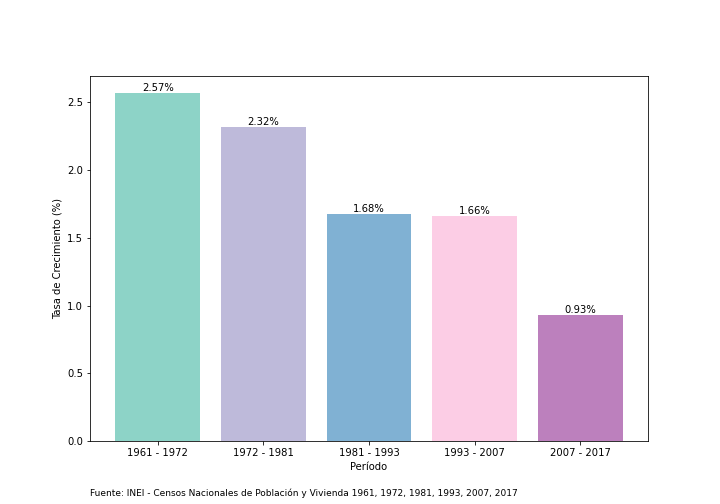
\includegraphics[scale=0.35]{tasas_crecimiento.png}
\caption{\textsc{Peru: Tendencia del Crecimiento Poblacional 1961 - 2017}}
\label{fig:1}
\end{figure}

\end{frame}


\subsection{4. El sistema de estadísticas vitales}
\begin{frame}{\textbf{4. El sistema de estadísticas vitales:}}
\justifying
\begin{block}{\textbf{4.1. Descripción de las estadísticas vitales y su importancia para el estudio demográfico.}}
\justifying
Las estadísticas vitales se refieren a los datos relacionados con los eventos vitales de la población, como nacimientos, defunciones, matrimonios y divorcios. Estas estadísticas son fundamentales para el estudio demográfico, ya que proporcionan información clave sobre la dinámica y la estructura de la población.

Las estadísticas vitales son importantes por varias razones:
\begin{enumerate}
\justifying
\item[A.] \textbf{Medición de la mortalidad:} Los datos sobre defunciones permiten calcular la tasa bruta de mortalidad, que es un indicador fundamental para evaluar la salud y el bienestar de una población. Estas estadísticas también permiten analizar las tasas específicas de mortalidad por edad, sexo y causas de muerte, lo que proporciona información valiosa para la planificación de servicios de salud y políticas de prevención.

\item[B.] \textbf{Análisis de la fecundidad:} Los datos sobre nacimientos y tasas de natalidad son esenciales para comprender los patrones de fecundidad en una población. Estas estadísticas permiten calcular indicadores como la tasa bruta de natalidad, la tasa general de fecundidad y la tasa de fecundidad por edad, lo que ayuda a identificar tendencias y variaciones en la fertilidad y a formular políticas de planificación familiar y salud reproductiva.
\end{enumerate}
\end{block}
\end{frame}

\begin{frame}{}

\begin{block}{}
\justifying
\begin{enumerate}
\justifying
\item[C.] \textbf{Evaluación de cambios demográficos:} Las estadísticas vitales son fundamentales para identificar cambios en la estructura demográfica de una población. Los datos sobre matrimonios y divorcios, por ejemplo, proporcionan información sobre los patrones de formación y disolución de parejas, lo que influye en la estructura familiar y en la composición de la población.

\item[D.] \textbf{Planificación y toma de decisiones:} Las estadísticas vitales son una herramienta crucial para la planificación y la toma de decisiones en diversos ámbitos, como la salud, la educación, la vivienda y la seguridad social. Estos datos permiten evaluar las necesidades de la población, identificar grupos vulnerables y diseñar políticas y programas que respondan de manera efectiva a las demandas demográficas.
\end{enumerate}
Es importante destacar que la calidad y la disponibilidad oportuna de las estadísticas vitales son esenciales para su utilidad en el estudio demográfico. Los sistemas de registro civil y los mecanismos de recolección de datos deben ser eficientes y confiables para garantizar la precisión de los resultados y permitir un análisis demográfico adecuado.
\end{block}
\end{frame}

\begin{frame}{}
\begin{block}{\textbf{4.2. Análisis de los principales eventos demográficos registrados en el sistema de estadísticas vitales, como nacimientos, defunciones, matrimonios y divorcios.}}
\justifying
El sistema de estadísticas vitales recopila y registra información sobre los principales eventos demográficos que ocurren en una población. Estos eventos incluyen nacimientos, defunciones, matrimonios y divorcios. A continuación, se presenta un análisis de cada uno de estos eventos:
\begin{enumerate}
\item[A)] \textbf{Nacimientos:}
\begin{itemize}
\justifying
\item[\ding{75}] Los datos sobre nacimientos son fundamentales para comprender la dinámica demográfica y la estructura de edad de una población. Estos datos proporcionan información sobre el crecimiento de la población y la fertilidad.
\item[\ding{75}] El análisis de los nacimientos incluye el cálculo de indicadores como la tasa bruta de natalidad, que representa el número de nacimientos por cada 1,000 habitantes en un año determinado.
\item[\ding{75}] Los datos de nacimientos también se utilizan para identificar patrones de fecundidad, como la edad media de la madre al momento del nacimiento y las tasas de fecundidad por grupos de edad.
\end{itemize}

\end{enumerate}
\end{block}
\end{frame}

\begin{frame}{}
\begin{block}{}
\justifying

\begin{enumerate}
\item[B)] \textbf{Defunciones:}
\begin{itemize}
\justifying
\item[\ding{75}] Los datos sobre defunciones son esenciales para el estudio de la mortalidad y la salud de la población. Estos datos proporcionan información sobre las causas de muerte y las tasas de mortalidad.
\item[\ding{75}] El análisis de las defunciones incluye el cálculo de indicadores como la tasa bruta de mortalidad, que representa el número de defunciones por cada 1,000 habitantes en un año determinado.
\item[\ding{75}] Los datos de defunciones también se utilizan para evaluar la esperanza de vida, que es una medida de la longevidad y refleja la media de años que se espera que viva una persona en una determinada población.
\end{itemize}
\item[C)] \textbf{Matrimonios:}
\begin{itemize}
\justifying
\item[\ding{75}] Los datos sobre matrimonios proporcionan información sobre los patrones de formación de parejas y las tendencias matrimoniales en una población.
\item[\ding{75}] El análisis de los matrimonios incluye el cálculo de indicadores como la tasa bruta de matrimonio, que representa el número de matrimonios por cada 1,000 habitantes en un año determinado.
\item[\ding{75}] Los datos de matrimonios también se utilizan para examinar la edad media al momento del matrimonio y las tasas de matrimonio por grupos de edad, lo que permite analizar las tendencias en la formación de parejas.
\end{itemize}
\end{enumerate}
\end{block}
\end{frame}


\begin{frame}{}
\begin{block}{}
\justifying

\begin{enumerate}
\item[B)] \textbf{Divorcios:}
\begin{itemize}
\justifying
\item[\ding{75}] Los datos sobre divorcios proporcionan información sobre las tasas de disolución de matrimonios y los patrones de divorcio en una población.
\item[\ding{75}] El análisis de los divorcios incluye el cálculo de indicadores como la tasa bruta de divorcio, que representa el número de divorcios por cada 1,000 habitantes en un año determinado.
\item[\ding{75}] Los datos de divorcios también se utilizan para examinar la duración media del matrimonio y las tasas de divorcio por grupos de edad, lo que permite analizar las tendencias en la estabilidad matrimonial.
\end{itemize}

\end{enumerate}
El análisis de estos eventos demográficos a través del sistema de estadísticas vitales proporciona información valiosa para comprender la dinámica y los cambios en la población, así como para informar la toma de decisiones en áreas como la salud, la planificación familiar y la política social. Además, permite monitorear la evolución de la estructura demográfica y evaluar el impacto de políticas y programas específicos en la población.
\end{block}
\end{frame}


\begin{frame}{}
\begin{block}{\textbf{4.3. Mención de cómo estos datos son utilizados para calcular indicadores demográficos, como tasas de natalidad, mortalidad y esperanza de vida.}}
\justifying
Los datos recopilados a través del sistema de estadísticas vitales son utilizados para calcular varios indicadores demográficos importantes. A continuación, se mencionan algunos ejemplos:
\begin{enumerate}
\justifying
\item[\ding{102}] \textbf{Tasa bruta de natalidad:} Se calcula dividiendo el número de nacimientos ocurridos en un año determinado por la población total y multiplicando el resultado por 1,000. Este indicador representa el número de nacimientos por cada 1,000 habitantes en un año y proporciona una medida general de la fecundidad de una población.
\item[\ding{102}] \textbf{Tasa bruta de mortalidad:} Se calcula dividiendo el número de defunciones ocurridas en un año determinado por la población total y multiplicando el resultado por 1,000. Este indicador representa el número de defunciones por cada 1,000 habitantes en un año y refleja la incidencia general de la mortalidad en una población.
\item[\ding{102}] \textbf{Esperanza de vida:} Se calcula utilizando los datos de defunciones y nacimientos para determinar la media de años que se espera que viva una persona en una determinada población. La esperanza de vida al nacer es un indicador ampliamente utilizado para evaluar la longevidad y la salud de una población.
\end{enumerate}
\end{block}
\end{frame}

\begin{frame}{}
\begin{block}{}
\justifying

\begin{enumerate}
\justifying
\item[\ding{102}] \textbf{Tasa de mortalidad infantil:} Se calcula dividiendo el número de defunciones de niños menores de un año ocurridas en un año determinado por el número de nacidos vivos en el mismo año y multiplicando el resultado por 1,000. Este indicador mide la probabilidad de que un niño muera antes de cumplir su primer año de vida y es utilizado para evaluar la salud y el bienestar infantil.
\item[\ding{102}] \textbf{Tasas de mortalidad específicas por edad y causa:} Utilizando los datos de defunciones, se pueden calcular tasas de mortalidad específicas por grupos de edad y causas de muerte. Estas tasas proporcionan información detallada sobre los patrones de mortalidad en diferentes segmentos de la población y permiten identificar las principales causas de muerte en una determinada área geográfica.
\end{enumerate}
Estos indicadores demográficos son de vital importancia para comprender la dinámica y la salud de una población. Permiten evaluar el impacto de factores como la fecundidad, la mortalidad y las condiciones de vida en el bienestar de las personas y sirven como base para la formulación de políticas y programas en áreas como la salud, la educación, la planificación familiar y la seguridad social.
\end{block}
\end{frame}

\subsection{5. Encuestas demográficas e información sobre movimientos espaciales}
\begin{frame}{\textbf{5. Encuestas demográficas e información sobre movimientos espaciales:}}
\begin{block}{\textbf{5.1. Explicación de las encuestas demográficas y cómo proporcionan información detallada sobre las características de la población.}}
\justifying
Las encuestas demográficas son herramientas de recopilación de datos utilizadas para obtener información detallada sobre las características de la población, como su composición socioeconómica, educativa, laboral, de salud, migratoria, entre otras. Estas encuestas se diseñan con el objetivo de obtener una muestra representativa de la población, lo que permite generalizar los resultados obtenidos a la población total.

Existen diferentes tipos de encuestas demográficas, como la Encuesta Nacional de Hogares, la Encuesta de Fecundidad y la Encuesta Nacional de Salud, entre otras. Cada una de estas encuestas se enfoca en recopilar datos específicos relacionados con su temática particular.

La recopilación de datos en las encuestas demográficas se realiza mediante entrevistas a los miembros de los hogares seleccionados en la muestra. Se utilizan cuestionarios estructurados que contienen preguntas sobre variables demográficas relevantes, como edad, género, nivel educativo, estado civil, ocupación, ingresos, entre otros. Estas preguntas permiten obtener información detallada sobre las características individuales y familiares de la población.
\end{block}
\end{frame}

\begin{frame}{}
\begin{block}{}
\justifying
Las encuestas demográficas proporcionan información valiosa para comprender la estructura y las dinámicas de la población. Al analizar los datos recopilados, se pueden obtener indicadores demográficos clave, como tasas de fecundidad, tasas de migración, tasas de empleo, tasas de alfabetización, entre otros. Estos indicadores permiten realizar análisis más precisos y detallados sobre la situación demográfica de un país o una región.

Además, las encuestas demográficas también permiten el estudio de las desigualdades sociales y la identificación de grupos de población que requieren intervenciones específicas. Por ejemplo, se puede identificar la prevalencia de la pobreza, las brechas educativas o las disparidades en el acceso a servicios de salud. Esta información es fundamental para la formulación de políticas y programas dirigidos a mejorar la calidad de vida de la población.

En resumen, las encuestas demográficas son una herramienta clave para obtener información detallada sobre las características de la población. Proporcionan datos que permiten analizar la estructura y las dinámicas demográficas, así como identificar desigualdades y orientar políticas y programas en beneficio de la sociedad.
\end{block}
\end{frame}

\begin{frame}{}
\begin{block}{\textbf{5.2. Análisis de la información sobre movimientos espaciales, como migraciones internas e internacionales, y su relevancia para el análisis demográfico.}}
\justifying
El análisis de la información sobre movimientos espaciales, como las migraciones internas e internacionales, es de gran relevancia para el estudio demográfico. Estos movimientos de población tienen un impacto significativo en la estructura y dinámica de las poblaciones, así como en diversos aspectos sociales, económicos y políticos. A continuación, se presenta un análisis de la importancia de esta información para el análisis demográfico:
\begin{enumerate}
\justifying
\item[A)] \textbf{Composición y distribución de la población:} El análisis de los movimientos espaciales permite comprender la composición y distribución de la población en diferentes áreas geográficas. Permite identificar las zonas de origen y destino de los migrantes, así como los flujos migratorios internos e internacionales. Esto es fundamental para comprender cómo se distribuye la población en un país o región, qué áreas experimentan crecimiento o declive poblacional, y cómo se relaciona con factores económicos, sociales y políticos.

\end{enumerate}
\end{block}
\end{frame}


\begin{frame}{}
\begin{block}{}
\justifying

\begin{enumerate}
\justifying

\item[B)] \textbf{Cambios en la estructura demográfica:} Los movimientos espaciales pueden influir en la estructura demográfica de una población. Por ejemplo, la migración puede afectar la proporción de hombres y mujeres en determinadas áreas, la distribución por edades y el tamaño de los grupos de población. Estos cambios demográficos tienen implicaciones importantes para la planificación de políticas sociales, educativas y de salud, así como para el diseño de programas de atención y servicios específicos.

\item[C)] \textbf{Determinantes y consecuencias de las migraciones:} El análisis de los movimientos espaciales proporciona información sobre los determinantes de las migraciones, como factores económicos, laborales, educativos, familiares o políticos. Además, permite estudiar las consecuencias de las migraciones tanto en las áreas de origen como en las de destino. Por ejemplo, se pueden analizar los efectos económicos de la migración en términos de remesas, impactos en el mercado laboral o cambios en la estructura productiva. Asimismo, se pueden evaluar los efectos sociales y culturales de las migraciones en términos de diversidad, integración, discriminación y cohesión social.
\end{enumerate}
\end{block}
\end{frame}


\begin{frame}{}
\begin{block}{}
\justifying

\begin{enumerate}
\justifying

\item[D)] \textbf{Políticas migratorias y gestión de la migración:} El análisis de los movimientos espaciales proporciona información relevante para la formulación y evaluación de políticas migratorias y la gestión de la migración. Permite comprender las tendencias migratorias, identificar los grupos vulnerables, evaluar el impacto de las políticas migratorias existentes y diseñar estrategias para abordar los desafíos asociados con la migración, como la protección de derechos, la integración socioeconómica y la gestión de la diversidad.
\end{enumerate}
En resumen, el análisis de la información sobre movimientos espaciales, como las migraciones internas e internacionales, es esencial para el estudio demográfico. Proporciona información clave sobre la composición, distribución y cambios en la estructura demográfica de las poblaciones, así como sobre los determinantes y consecuencias de las migraciones. Además, contribuye a la formulación de políticas migratorias y la gestión adecuada de la migración.
\end{block}
\end{frame}

\subsection{6. Las encuestas por muestreo}
\begin{frame}{\textbf{6. Las encuestas por muestreo:}}
\begin{block}{\textbf{6.1. Definición y características de las encuestas por muestreo.}}
\justifying
Las encuestas por muestreo son una técnica utilizada en investigación y recopilación de datos que permite obtener información representativa sobre una población objetivo a través de la selección de una muestra. En lugar de encuestar a toda la población, se elige una muestra representativa y se recopilan datos de los individuos o unidades seleccionadas en esa muestra. A continuación, se presentan las características principales de las encuestas por muestreo:
\begin{enumerate}
\justifying
\item[A.] \textbf{Representatividad:} La muestra seleccionada en una encuesta por muestreo debe ser representativa de la población objetivo. Esto significa que cada individuo o unidad en la población debe tener una probabilidad conocida y no nula de ser seleccionado en la muestra. De esta manera, los resultados obtenidos de la muestra pueden generalizarse con cierta confianza a toda la población.
\item[B.] \textbf{Aleatoriedad:} La selección de la muestra se realiza mediante un proceso aleatorio, lo que significa que cada individuo o unidad de la población tiene la misma oportunidad de ser seleccionado. Esto asegura que no exista sesgo en la selección y que todos los segmentos de la población tengan la posibilidad de ser representados en la muestra.
\end{enumerate}
\end{block}
\end{frame}

\begin{frame}{}
\begin{block}{}
\justifying

\begin{enumerate}
\justifying
\item[C.] \textbf{Tamaño de la muestra:} El tamaño de la muestra en una encuesta por muestreo debe ser lo suficientemente grande para garantizar la precisión de los resultados. El tamaño de la muestra se determina teniendo en cuenta la variabilidad de las características de interés en la población, el nivel de confianza deseado y el margen de error aceptable.
\item[D.] \textbf{Diseño muestral:} El diseño de la muestra puede ser de diferentes tipos, como muestreo aleatorio simple, muestreo estratificado, muestreo por conglomerados o muestreo sistemático, entre otros. Cada tipo de diseño tiene sus propias ventajas y se utiliza en función de las características de la población y los objetivos de la encuesta.
\item[E.] \textbf{Recopilación de datos:} Una vez seleccionada la muestra, se lleva a cabo la recopilación de datos a través de entrevistas personales, cuestionarios en línea, llamadas telefónicas u otros métodos. Es importante seguir un protocolo estandarizado para asegurar la consistencia en la recopilación de datos y minimizar los sesgos o errores de medición.
\end{enumerate}
\end{block}
\end{frame}

\begin{frame}{}
\begin{block}{}
\justifying

\begin{enumerate}
\justifying
\item[F.] \textbf{Análisis de datos:} Una vez recopilados los datos de la muestra, se realiza el análisis estadístico para obtener resultados descriptivos y estimaciones de los parámetros de interés en la población objetivo. Se utilizan técnicas estadísticas apropiadas para tener en cuenta el diseño muestral y calcular los intervalos de confianza de las estimaciones.
\end{enumerate}
Las encuestas por muestreo son ampliamente utilizadas en diferentes áreas de estudio, incluyendo la demografía, la economía, la sociología, la salud y muchas otras disciplinas. Permiten obtener información valiosa de manera eficiente y representativa, lo que facilita la toma de decisiones y la formulación de políticas basadas en evidencia. Sin embargo, es importante tener en cuenta las limitaciones inherentes a este método, como posibles errores de muestreo y no respuesta, y aplicar técnicas adecuadas para minimizar su impacto en los resultados.
\end{block}
\end{frame}

\begin{frame}{}
\begin{block}{\textbf{6.2. Explicación de cómo se selecciona una muestra representativa y cómo se obtienen estimaciones para la población en general.}}
\justifying
La selección de una muestra representativa en una encuesta por muestreo implica seguir un proceso riguroso para garantizar que los resultados obtenidos sean generalizables a la población en general. A continuación, se describe el procedimiento general para seleccionar una muestra representativa y obtener estimaciones para la población:
\begin{enumerate}
\justifying
\item[A)] \textbf{Definición de la población objetivo:} El primer paso es definir claramente la población objetivo de la encuesta. Esto implica especificar las características demográficas, geográficas u otras que se desean estudiar y sobre las cuales se desean obtener estimaciones.
\item[B)] \textbf{Determinación del tamaño de la muestra:} A partir de la población objetivo, se debe determinar el tamaño adecuado de la muestra. El tamaño de la muestra depende de la variabilidad de las características en la población, el nivel de confianza deseado y el margen de error aceptable. Generalmente, se utiliza un enfoque estadístico para calcular el tamaño de la muestra que asegure una precisión adecuada de las estimaciones.
\end{enumerate}
\end{block}
\end{frame}

\begin{frame}{}
\begin{block}{}
\justifying
\begin{enumerate}
\justifying
\item[C)] \textbf{Elección del diseño de muestreo:} Se selecciona el diseño de muestreo más apropiado para el estudio. Los diseños de muestreo comunes incluyen el muestreo aleatorio simple, el muestreo estratificado, el muestreo por conglomerados y el muestreo sistemático. Cada diseño tiene sus propias características y se utiliza en función de la estructura de la población y los objetivos de la encuesta.
\item[D)] \textbf{Selección de la muestra:} Una vez definido el diseño de muestreo, se procede a la selección de la muestra. La selección se realiza de manera aleatoria, asegurando que cada elemento de la población objetivo tenga una probabilidad conocida y no nula de ser seleccionado. Esto se logra mediante técnicas como el muestreo aleatorio simple, el muestreo estratificado proporcional, el muestreo por conglomerados en etapas, entre otros.

\item[E)] \textbf{Recopilación de datos:} Una vez seleccionada la muestra, se procede a la recopilación de datos. Esto puede implicar la realización de entrevistas personales, la distribución de cuestionarios en línea, la recopilación de registros administrativos u otros métodos de recolección de datos. Es importante seguir un protocolo estandarizado para asegurar la consistencia en la recopilación de datos.
\end{enumerate}
\end{block}
\end{frame}


\begin{frame}{}
\begin{block}{}
\justifying
\begin{enumerate}
\justifying
\item[F)] \textbf{Análisis de datos y estimaciones:} Una vez que se recopilan los datos de la muestra, se realiza el análisis estadístico. Esto implica calcular estimaciones puntuales y estimaciones de intervalo para las características de interés en la población. Se utilizan técnicas estadísticas apropiadas que toman en cuenta el diseño de muestreo, como los pesos muestrales y las fórmulas de estimación adecuadas, para garantizar que las estimaciones sean representativas de la población objetivo.
\end{enumerate}
Al seguir estos pasos, es posible obtener estimaciones confiables y generalizables para la población en general utilizando una muestra representativa. Sin embargo, es importante tener en cuenta las limitaciones inherentes al muestreo, como el error de muestreo y la no respuesta, y aplicar técnicas adecuadas para minimizar su impacto en los resultados.
\end{block}
\end{frame}


\begin{frame}{}
\begin{block}{\textbf{6.3 Ejemplos de encuestas por muestreo utilizadas en el estudio demográfico.}}
\justifying
Existen varias encuestas por muestreo utilizadas en el estudio demográfico. A continuación, se presentan algunos ejemplos de encuestas por muestreo comúnmente utilizadas en este campo:
\begin{enumerate}
\justifying
\item[\ding{79}] \textbf{Encuesta Nacional de Demografía y Salud (ENDES):} Es una encuesta por muestreo que se realiza en varios países, incluido Perú. Recopila información sobre diferentes aspectos de la salud y la demografía, como la fecundidad, la mortalidad, el uso de anticonceptivos, la atención prenatal y el acceso a servicios de salud. La ENDES proporciona datos detallados sobre indicadores demográficos clave y características de la población.

\item[\ding{79}] \textbf{Encuesta Nacional de Empleo e Ingresos (ENEI):} Esta encuesta por muestreo se enfoca en aspectos relacionados con el empleo y los ingresos de la población. Proporciona información sobre la tasa de desempleo, la ocupación laboral, los ingresos familiares y otros indicadores relacionados con el mercado laboral. Estos datos son relevantes para el análisis demográfico, ya que permiten comprender la estructura y dinámica de la población activa.

\end{enumerate}
\end{block}
\end{frame}

\begin{frame}{}
\begin{block}{}
\justifying
\begin{enumerate}
\justifying
\item[\ding{79}] \textbf{Encuesta Nacional de Hogares (ENAHO):} Esta encuesta por muestreo recopila información sobre diversos aspectos socioeconómicos de los hogares, incluidos la estructura familiar, la vivienda, la educación, la pobreza y el acceso a servicios básicos. Los datos obtenidos de la ENAHO permiten analizar la composición y las características de los hogares, lo cual es fundamental para comprender las dinámicas demográficas de la población.

\item[\ding{79}] \textbf{Encuesta Demográfica y de Salud Familiar (DHS):} Esta encuesta por muestreo se lleva a cabo en varios países y proporciona información detallada sobre la salud y la demografía, centrándose en temas como la fecundidad, la mortalidad infantil, la planificación familiar, el uso de servicios de salud materna e infantil, entre otros. Los datos de la DHS son utilizados para evaluar el impacto de políticas y programas relacionados con la salud y el bienestar de la población.

\item[\ding{79}] \textbf{Encuesta Continua de Hogares (ECH):} Es una encuesta por muestreo que se realiza de forma continua y periódica en algunos países. Proporciona información sobre diversos aspectos demográficos y socioeconómicos de los hogares, como el empleo, la educación, los ingresos, la vivienda y la migración. Los datos de la ECH permiten analizar las tendencias y cambios en las características de la población a lo largo del tiempo.
\end{enumerate}
\end{block}
\end{frame}

\begin{frame}{}
\begin{block}{}
\justifying
Estos son solo algunos ejemplos de encuestas por muestreo utilizadas en el estudio demográfico. Cada una de estas encuestas recopila información específica que permite comprender diferentes aspectos de la población y su dinámica demográfica. La selección de la encuesta adecuada depende de los objetivos de investigación y las variables de interés en el análisis demográfico.
\end{block}
\end{frame}


\begin{frame}{\textbf{Referencias Bibliográficas}}

\begin{itemize}
\justifying
\item Coale, A. J., \& Hoover, E. M. (2019). Principios de demografía histórica. Siglo XXI Editores.
\item Durán, R., \& Piña, J. (2014). Introducción a la demografía. El Colegio de México.
\item León Castillo, L. A. (2015). Análisis Económico de la Población. Demografía.
\item López-Casanovas, G., \& Rivera, B. (2010). La demografía económica. Alianza Editorial.
\item Pérez Díaz, V. (2016). Demografía general. Pirámide.
\item Romero, D. M., \& Lamas, A. (2014). La demografía en México: un campo en transformación. El Colegio de México.
\item Santacreu, O. (2015). Introducción a la demografía histórica. Ediciones Octaedro.
\item Silber, D. (2014). Demografía: una ciencia para el siglo XXI. Siglo XXI Editores.
\item Tabutin, D., \& Schoumaker, B. (2017). Demografía: conceptos y mediciones. El Colegio de México.
\item Zamora, M. J. (2015). Demografía: una introducción. Editorial UOC.
\end{itemize}

\end{frame}

}
\end{document}